\documentclass[12pt]{article} 
\setlength{\paperheight}{11in}

%Margins: 
\usepackage{geometry} 
\geometry{top=1.0in, bottom=1.0in, left=1.25in, right=1.25in} 

%Header 
\usepackage{fancyhdr}
\setlength{\headheight}{15pt} \pagestyle{fancyplain}\lhead{\small{Part \thepart}}
\rhead{\fancyplain{}{\small{\textit{\leftmark}}}}\cfoot{\small{\thepage}}

%Font {Options are sfdefault or rmdefault for roman orsans-serif} 
\renewcommand{\familydefault}{\sfdefault} 

%Import Packages: 
\usepackage{amsmath, amssymb, graphicx, fontenc,color,setspace, ulem} 

%To insert PDFs (For Appendix):
\usepackage[final]{pdfpages} 

\begin{document} 
%Include the Opening (Title, Abstract, etc)

\begin{titlepage}
\pagestyle{plain}
\lhead{}
\rhead{}
\cfoot{Carroll College 2012\\Mathematics, Computer Science, \& Engineering}
% ---------------- TITLE PAGE ------------------%
\title{CS 430: Senior Project\\Robotics}
\author{\small{Students}\\
Nathan Woods,  Jennings Anderson \\Shae Tiegen,  Forrest Laskowski\\[2mm]
\small{Professor}\\
Steve Harper}
\date{\small{Term}\\
Spring 2012}
\maketitle

%---------------- ABSTRACT -------------------%
\begin{abstract}
This documentation outlines the Robot built for CS 430: Senior Project in spring 2012.  It first outlines the semester's work and project goals.

It is written such that one should be able to reconfigure a similar robot to run this code and understand the logic.

There are directions for setting up a development environment to interface with the IntelliBrain2 MicroController in order to load the software with a detailed description and sample load script.

A physical description and a wiring diagram should allow for another student one day to reconstruct a similar robot.

Ultimately, this documentation outlines each piece of logic that controls the robot and describes specific nuances in the logic and the processes that the authors went through.

The authors believe the robotics project to be a great success and good learning opportunity.  Though the robot's navigation skills are currently poor, both it and the developers are young in the art of robotics and hold high hopes for future releases of the robot, dubbed `Dufus.'

\end{abstract}
\end{titlepage}

\newpage
\setcounter{page}{1}
\pagenumbering{roman}
%Header
\pagestyle{fancyplain}
\rhead{\fancyplain{}{\small{\textit{SIGNATURE PAGE}}}}
\cfoot{\small{\thepage}}
\clearpage

%------------TABLE OF CONTENTS ---------------%

%Header
\pagestyle{fancyplain}
\rhead{\fancyplain{}{\small{\textit{TABLE OF CONTENTS}}}}
\cfoot{\small{\thepage}}
\singlespace
\tableofcontents

%And then clear for a new page.
\clearpage
\onehalfspacing

%%%%%%%%%%%%%%%%%%%%%%%%%%%%% BEGIN CONTENT %%%%%%%%%%%%%%%%%%%%%%%%%%%%%%\
\setcounter{page}{1}
\pagenumbering{arabic}
%Header 
\setlength{\headheight}{15pt} \pagestyle{fancyplain}\lhead{\small{\textit{SENIOR PROJECT 2012}}}
\rhead{\fancyplain{}{\small{\textit{\leftmark}}}}\cfoot{\small{\thepage}}
\section{Introduction}
--Discuss here what the documentation is about and how to use it.

\clearpage
\section{Development Environment}
The IntelliBrain2 can be programmed in Java.  A specific RoboJDE library is required at compile to interface with the board.  There are numerous options to turn Java code into running code on the robot, we will explain them here.
\subsection{Requirements}
First, download the development software from the Ridgesoft Website:\\
{\color{blue}\centerline{http://ridgesoft.com/robojde/robojde.htm}}\\
The software, API, required libraries, and physical wiring diagrams can be found on this website.

There is an included development application, \textit{RoboJDE}, that uses RoboJDE project files $(.rjp)$ to program the robot.  This editor is great for getting started.  The software comes with many example files and as long as the host computer has a Serial Port (We used an OptiPlex GX620), then there is no additional software required to get the first programs loaded to the robot.

One will quickly outgrow this environment for programming because it is all plain text with no syntax coloring or error detection.  We found Eclipse to be the best editor because it can be configured to automatically compile to the robot using the rsload script.

\subsection{RSLoad Script}
Included in downloads for all platforms is a script called rsload.  rsload is a command line utility for loading code to the robot.  The best documentation on it can be found here:\\
{\color{blue}\centerline{http://ridgesoft.com/robojde/2.0/docs/RoboJDEGuide.pdf}}
Some important arguments to know are:
\begin{description}

\item[-port] Specifies the port the robot is connected to, typically COM1 on Windows or /dev/ttys0 on Linux, but if using a USB adapter, this could be /dev/tty.usbserial or COM5.  Understanding particular drivers and the OS is important here.
\item[-run] If included, the robot will automatically run when load is complete.
\item[-bank] Specify to load to either Flash or Ram; we always loaded to Flash and in some cases, it was required to use this argument.
\item[-verbose] Good for debugging purposes.
\end{description}

The ultimate required argument is the name of the class that includes main.  An example call:
\begin{verbatim}
rsload -bank Flash -port /dev/tty.usbserial -run Controller
\end{verbatim}
This command will load the Controller class to the robot over the USB to Serial adapter.  When load is complete, it will run the program.  It should be noted that in this example, Controller.class is located in the same directory as rsload.

\subsection{Individual Load Scripts}
For greater compatability, we wrote a customizable load scirpt that would compile and then load a specific file, given the file path and the name of the file containing the function, $main$.
\small{\begin{verbatim}
#Instructions:
#Update both filePath and fileName variables to represent where the files are.
#These should all be relative to Dropbox.  (Note in eclipse cases, compiled files 
#may be found in the /bin/ directory of the project.  However, these should be 
#pointed to the java file for compiling.
#Don't put a '/' on the end of the filePath:
#The fileName is the main controlling class.
#Warning! Every .java file in the path BETTER compile.
#This is an example:
#filePath=/home/robotics/Dropbox/Robo/Development/Forrest
#fileName=MusicTest
###############################################################
####################### WHAT YOU SHOULD EDIT ####################
filePath=/home/robotics/Dropbox/Robo/Development/Master/Robot/src 
#Note, don't end with /
fileName=Controller		#Note, no .java or .class! This has 'main function'
######################## END WHAT YOU SHOULD EDIT ###############
###############################################################
clear
echo "Welcome to the CS 430 Load Script"
echo "This will fail if RoboJDE is running"
echo ""
echo "Copying to Temp Build Path to not upset Eclipse..."
rm -f /home/robotics/Dropbox/Robo/Development/TempLoadNoTouchie/*
cp $filePath/* /home/robotics/Dropbox/Robo/Development/TempLoadNoTouchie/
echo "Files Copied To Temp Build Path:"
cd /home/robotics/Dropbox/Robo/Development/TempLoadNoTouchie
ls -al
echo "Press Enter to Compile"
read nothing
#Let's compile it first:
echo "Compiling..."
javac -classpath "/home/robotics/RoboJDE/RoboJDE.jar" *.java
echo "Compilation Complete"
echo "Make sure Robot is in Bootstrap Mode, Turn ON then press STOP, 
                                                   Then Press Enter"
read nothing
echo "Initiating Robot Loader:"
sh /home/robotics/RoboJDE/rsload -port /dev/ttyS0 -bank flash $fileName
echo ""
echo "Press Enter to Quit"
read nothing
\end{verbatim}}

This script was written for the robotics user account on an OptiPlex GX620 running Ubuntu 11.10 with the robot connected to the serial port.  It will copy the required files to a temporary directory, compile them and then load them to the robot.

The main purpose of a script like this is to abstract the robot development to simple java files in a single directory.  The script takes care of including the necessary files for interfacing with the board, so the user can write simple Java code to feed this script.

Next, we take this concept one step further by integrating with Eclipse.

\subsection{Integrating with Eclipse}
Eclipse is a robust open source development environment that allows for much customization.  The two requirements for this project are:
\begin{enumerate}
\item Include the RoboJDE.jar archive in the compile path
\item Write an external build tool to automatically call the rsload script.
\end{enumerate}

Once a project is created in Eclipse, preferences can be set by right-clicking on the project root.  Ensure here that the Java Build Path includes the RoboJDE.jar file.  It is convenient to put a copy of this file in the workspace directory so that it can be referenced locally.

There are explicit instructions for setting up an eclipse external tool in the read me, but I have included a screen shot here for further description:
\clearpage
\begin{figure}[h]
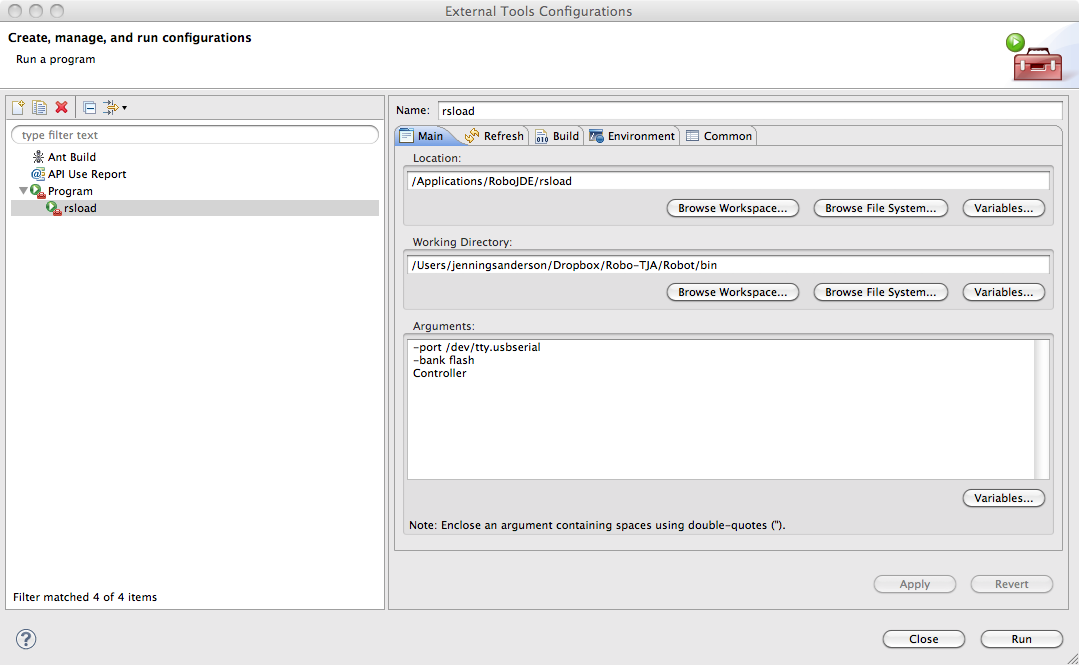
\includegraphics[scale=.4]{img/externalTool}
\caption{Eclipse External Tool Configuration}
\end{figure}

This tool configuration differs from the suggested configuration with static references for convenience.  Note that the Working Directory references the bin directory, where Eclipse puts the compiled class files.  The name of the class with the function, $main$ in it is $Controller$.

\subsection{Source Version Control}
The importance of a steadfast source version control method should not be over looked; unfortunately, we did so for months until turning to git and github.com.  We recommend to spend the time in the beginning 

\subsubsection*{SVC Anecdote}
While Dropbox is a simple, convenient, and magical application in today's computing, it is not a substitute for source version control.  We initially used Dropbox to sync files across all of our computers for team development.  The problem here is that changes propagate immediately.  Backups are kept in the depths of Dropbox's servers, but are tedious to scan through and recover.  However, the real kicker occurs when Dropbox meets DeepFreeze, the Enterprise software that Carroll uses to fight malicious intentions.  If Dropbox is installed on a user's profile, it will by default sync all files to a folder on the local hard drive.  When the computer restarts, changes to the $C$ drive are erased and Dropbox is fooled into believing the user deleted all files in their Dropbox directory.  This change is then propagated to the rest of the team, so come Monday morning, all code is erased across every team member's computer.  \textit{Thanks, Forrest}.

\clearpage
\section{Robot}

\section{Robot}

\section{Logic}

\section{Conclusion}

\end{document}